% This is a default-selection of plugins that are used widely in this repo.

\documentclass[a4paper,10pt,fleqn]{article}
\usepackage[utf8]{inputenc}

% deutsche Trennmuster etc.
\usepackage[ngerman]{babel}
\usepackage[T1]{fontenc}

% mathematical simbols and fonts
\usepackage{mathtools} 
\usepackage{amssymb}
\usepackage{amsmath}
\usepackage{ntheorem}
\usepackage{polynom}
\usepackage{marvosym}
\usepackage{tabu}
\renewcommand*{\bmod}{\mathbin{\%}}
\everymath{\displaystyle}

\usepackage{multicol}
\usepackage{color}
\usepackage[usenames,dvipsnames]{xcolor}
\setlength{\columnsep}{1cm}
\setlength{\columnseprule}{0.25pt}
\def\columnseprulecolor{\color{gray}}
\usepackage{hyperref}

\usepackage[margin=1.5cm]{geometry}
\usepackage{graphicx}
\usepackage{pgfplots}
\pgfplotsset{compat=1.10}

%Code higlighting

\usepackage{minted}

% make lists more compact:
\newlength{\wideitemsep}
\setlength{\wideitemsep}{.5\itemsep}
\addtolength{\wideitemsep}{-5pt}
\let\olditem\item
\renewcommand{\item}{\setlength{\itemsep}{\wideitemsep}\olditem}
\renewcommand{\arraystretch}{1.25}

\title{Zusammenfassung AutoSpr}
\author{Fabian Hauser}
 
\begin{document}
\maketitle

\section{Varia}
Unterrichtszeiten: 12:00-12:30, 13:45-14:15, 14:20-14:50

Prüfung: Zusammenfassung $1m^2  = 8 \cdot A4$, Taschenrechner


\section{Notation}
Prädikat:	Aussagen

\subsection{Logik}
Siehe Seite 5 Script!

\subsection{Mengenlehre}

\section{Sprachen}

\subsection{Alphabet}
Definition : Nicht leere Menge von "Zeichen".

Zum Beispiel: $\Sigma = \{0, 1\}$, $\Sigma = \{1\}$, $\Delta = \{a,b,c,...,z\}$


\subsection{Wort}

Definition: Zeichenkette von Zeichen aus $\Sigma$: $w \in \Sigma^n = \Sigma \times \Sigma \times ... \times \Sigma$. Länge: $|w| = n$
\[
	\Sigma^0 = \{\epsilon\}; \epsilon = \text{ leeres Wort}
\]
\[
	\Sigma^\ast = \Sigma^0 \cup \Sigma^1 \cup ... \cup \Sigma^n = \bigcup^{\infty}_{k=0}{\sum^k}
\]

Im Zusammenhang mit der Sprache sind Zeichenketten bedeutungslos!

\paragraph{Beispiele}

\begin{align*}
	\Sigma &= \{1\} & \Sigma^\ast &= \{\epsilon, 1,11,111,1111,...\} \\
	L &\subset \Sigma^\ast  & L &=\{1,11,1111,11111111,....\} = \{w \in \Sigma^\ast| |w|=2^k, k \in \mathbb{N}\}
\end{align*}


\subsection{Notationen}
Beispiele:
\begin{align*}
	\Sigma &= \{0,1\} \\
	L_1 &= \{0^n 1^n | n \geq 0\} &\rightarrow 0^n = 00...0 \\
	L_2 &= \left\{ w \in \Sigma^\ast \left| \left|w\right|_0 = \text{ Anzahl 0 in } w = \left|w\right|_1 \right.\right\} \\
	L_3 &= \left\{w \in \Sigma^\ast \left| \text{ Zahlenwert von } w \text{ ist durch 3 teilbar} \right.\right\}
\end{align*}

Sprache für Graphen:

\begin{align*}
V & \text{ Vertices} \\
E & \text{ Edges} &= \{a,b\}, a,b \in V \\
G &= (V, E) &= (\{0,1,9,27\},\{\{0,1\},\{1,3\},\{1,27\},...\}) \\
\Sigma &= \left\{\ (,),",","\{","\}", 0, 1,2,...,9 \right\}
\end{align*}
jeder Graph lässt sich so codieren: $g \subset \Sigma^\ast, g = \{w \in \Sigma^\ast \left| w \text{ ist eine Graph-Beschreibung} \right.\}$

\section{Endliche Automaten und reguläre Sprachen}

Bei einem endlichen Automat braucht es für den ganzen Gültigkeitsbereich gültige Zustände / Pfeile.

\paragraph{Beispiel: Drehkreuz Skilift, ein deterministischer endlicher Automat}

	Zwei Zustände: Verriegelt / Entriegelt
	
	Drehen und Fahrkarten ändern den Zustand.
	
	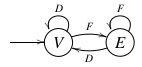
\includegraphics[scale=0.5]{img/skilift.png}

Zutaten: 

\begin{align*}
	A	&= (Q, \Sigma, \delta, q_0, F)  \\
	Q	&= \text{ Zustände} \\
	\Sigma	&= \text{ Alphabet} \\
	\delta	&= \text{ Übergangsfunktion (Pfeile)} \\
	q_0	&\in Q \text{, Startzustand (Initialisierung)} \\
	F	&\subset Q \text{, Akzeptierzustand}
\end{align*}

Zeichenbedeutungen:

$\delta$: Zustand, Zeichen $\rightarrow$ neuer Zustand.

$(q, a) \mapsto q'=\sigma(q,a)$

%$Q \multiply \Sigma \rightarrow^{\sigma} Q$

\subsection{Darstellung mittels Tabelle}

\begin{tabular}{c c}
 & $\Sigma$ \\
$Q$	& $\delta$
\end{tabular}

\subsection{Systematische Rekonstruierung aus der Sprache}

Zustände sind charakterisiert durch "was noch kommen darf"

\begin{align*}
	L(w) = \{v \in \Sigma^\ast | wv \in L \} \\
	\text{Beispiel: } \Sigma = \{a, b \}, L=\{ w \in \Sigma^\ast | |w|_a \text{ gerade}\}
\end{align*}


%TODO: Myhill-Nerode Tabelle mit Zuständen

\begin{align*}
W & L(w) \text{ (was kann angehängt werden)}\\
\epsilon & L(\epsilon) = \{v \in \Sigma^\ast | \epsilon v \in L \} &= L \\
a & L(a) = \{v \in \Sigma^\ast | a v \in L \} &= \{ v \in \Sigma^\ast | |w|_a ungerade \}\\
b & L(b) = \{v \in \Sigma^\ast | b v \in L \} &= L\\
  & L(aa) &= L \\
  & L(ab) &= L(a) \\
  & L(ba) &= L(a) \\
  & L(bb) &= L
\end{align*}

\begin{enumerate}
	\item $L(w)$ ausrechnen: verschiedene $L(w)$ geben $Q$ 
	\item $\sigma: L(w) \rightarrow^a L(wa)$
	\item $q_0: L(\epsilon) = L$
	\item $L(w)$ ist Akzeptierzustand wenn $\epsilon \in L(w)$
\end{enumerate}

\subsection{Gleichheit von Automatensprachen feststellen}
	Reduktion auf Minimalautomat M$(A_1)$. Vereinfachung geht, indem zuerst die nicht-Equivalenten zuständige gemäss folgender Liste ausgeschlossen werden:

\begin{enumerate}
	\item Akzeptierzustand $\neq$ Nicht-Akzeptierzustand 
	\item Führt am $m$ Zustände $m$ ein nicht äquivalentes Paar über.
	\item Wiederholung des Algorithmus, bis keine Änderungen mehr auftreten.
	\item Restliche Zustände sind äquivalent.üü
\end{enumerate}

\section{Stachoautomaten}

\section{Turing-maschinen}

\end{document}